\section{Problema 1: Saliendo del Freezer}

\subsection{Descripción de la problemática}
Este problema modela un edificio de N pisos (y planta baja) en el cual en vez de tener escaleras o ascensores, hay portales que lo transportan a uno desde un piso a otro. Los portales solo permiten ascender de un piso más bajo a uno más alto. En cada piso puede haber cualquier cantidad de portales, teniendo en cuenta que no hay dos portales que salgan del mismo piso y lleguen a un mismo piso. Todas las instancias del problema deben tener al menos un camino de portales entre la planta baja y el piso N.

Se pide diseñar un algoritmo de complejidad O($n^{2}$) que encuentre un camino que llegue desde planta baja hasta el piso N y utilice la mayor cantidad de portales posible.

El formato de entrada es un archivo de texto. Cada problema está representado en dos líneas de texto. La primera es el valor de N. La segunda es una lista de portales que sigue el siguiente formato:

\begin{verbatim}
pd ph[; pd ph]    // pd (piso desde), ph (piso hasta) enteros, pares de p separados por "; "
\end{verbatim}

Para la salida, lo único que interesa es la cantidad de portales que hay que utilizar para recorrer el camino que usa la cantidad máxima posible de portales. La salida es una línea de texto que tiene ese valor.


Por ejemplo, un edificio de cinco pisos que tiene, desde cada piso, un portal para llegar a todos los pisos superiores se escribiría de este modo en el formato de entrada:

\begin{verbatim}
5
0 1; 0 2; 0 3; 0 4; 0 5; 1 2; 1 3; 1 4; 1 5; 2 3; 2 4; 2 5; 3 4; 3 5; 4 5;
\end{verbatim}

Y el resultado a este ejemplo es, por supuesto, 5, ya que el camino más largo es el que pasa por todos los pisos.


\subsection{Algoritmo desarrollado}


El algoritmo diseñado utiliza la técnica de programación dinámica con un enfoque \textit{bottom-up}. Podemos subdividir el problema original en sub-problemas. Los subproblemas implican resolver lo mismo pero, en vez de partiendo desde la planta baja, partiendo desde un piso más alto. Cuanto más cercano al piso superior (N) esté el piso desde el que partimos, más chico es el subproblema.

En primer lugar \textit{parseamos} los datos de entrada, generando una tabla de tamaño N. La tabla contiene una lista de enteros en cada posición. La lista que se encuentra en la posición i-ésima de la tabla representa a los portales que salen desde el piso i. Los valores de la lista son los pisos a los que se llega desde ese piso usando un portal.

Luego, inicializamos en \texttt{-1} una tabla de resultados parciales. Nos referimos a resultados parciales porque en la posición i-ésima de la tabla resultados encontraremos la respuesta al subproblema de ``máxima cantidad de portales que se pueden utilizar para llegar al piso N partiendo desde el piso i''. Si no es posible llegar al piso N desde el piso i, guardaremos el valor -1 en esa posición.

Nótese que ninguna de las dos tablas tiene un lugar para el piso N, ya que no hay portales que partan desde el piso N ni tiene sentido el problema de llegar al piso N desde el mismo piso N.

Finalmente, el algoritmo itera por cada piso del edificio desde el piso $N-1$ hasta el 0, iterando en cada piso por todos los portales del piso. Para cada portal calculamos la cantidad máxima de portales que se pueden usar para llegar a N usando ese portal. Esto se hace en tiempo constante, ya que hay que verificar solo tres cosas: 

\begin{enumerate}[label*=\bfseries\arabic*.]
 \item leer el valor de N del archivo de entrada
 \item inicializar la tabla \texttt{portales} con listas (de enteros) vacías
 \item inicializar la tabla \texttt{resultados} con \texttt{-1}
 \item llenar la tabla \texttt{portales} con los portales de cada piso
 \item Para cada piso \texttt{p} desde $N-1$ hasta 0:
 \begin{enumerate}[label*=\bfseries\arabic*.]
    \item Inicializar variable \texttt{MAX} en -1
    \item Para cada portal \texttt{l} en \texttt{portales[p]}:
    \begin{enumerate}[label*=\bfseries\arabic*.]
      \item inicializamos una variable \texttt{costo} en -1 para representar la máxima cantidad de portales que se pueden utilizar para llegar a N usando el portal \texttt{l}
      \item Tenemos tres opciones:
      \begin{enumerate}[label*=\bfseries\arabic*.]
	\item Si el portal va directo a N, el costo es 1
	\item Si el portal va a un piso que tiene en la tabla \texttt{resultados} valor -1, no es posible llegar a N usando ese portal, y dejamos el costo en -1
	\item Finalmente, si el portal va a un piso que tiene en la tabla \texttt{resultados} un valor distinto a -1, entonces el costo será ese valor + 1 (por el portal \texttt{l})\footnote{Nótese que, como los portales siempre van a pisos más alto, las posiciones de \texttt{resultados} de los pisos más altos ya van a haber sido completadas en iteraciones anteriores del algoritmo.} 
      \end{enumerate}

      \item Ahora que ya tenemos el costo, si el costo obtenido para este portal es mayor a la variable \texttt{MAX}, actualizamos el valor de ésta con el costo obtenido en esta iteración
    \end{enumerate}
    \item Guardar en \texttt{resultados[p]} en valor de \texttt{MAX}
 \end{enumerate}
 \item El resultado del problema completo se encontrará en \texttt{resultados[0]}
\end{enumerate}


\subsection{Tests de correctitud}


Los casos de test provistos por la cátedra fueron replicados en el script \texttt{test.sh}. Para correrlo, primero es necesario tener el código del ejercicio compilado, lo cual se hace ejecutando el comando \texttt{make} en el directorio del código fuente.


\subsection{Análisis de la complejidad}

En en código fuente hemos comentado las distintas partes indicando los costos de cada una. Si llamamos $N$ a la cantidad de pisos del edificio y $P$ a la cantidad total de portales, la conclusión a la que llegamos es que el algoritmo tiene un costo de $\mathcal{O}(N+P)$. 

Ahora bien, la cantidad de portales pertenece a $\mathcal{O}(N^2)$. En un edificio con la máxima cantidad posible de portales tendremos N portales en el piso 0, N-1 portales en el piso 1, etc. hasta el piso N-1, donde tendremos un solo portal. Esa sumatoria se escribe de este modo:

$\displaystyle\sum_{i=1}^{N} i = \frac{N (N+1)}{2} = \frac{N^2 + N}{2}$

Por lo tanto, podemos reescribir el costo del algoritmo en función de $N$ como perteneciente a $\mathcal{O}(N+N^2)$, lo cual pertenece a $\mathcal{O}(N^2)$, que es lo que se pide en el enunciado.

\newpage

\subsection{Código fuente}
\lstinputlisting[name=Solucion, numbers=left, frame=lines, firstline=139, lastline=165]{../src/ej1/ej1.cpp}

\subsection{Medición empírica de la complejidad}

Para la medición de tiempos agregamos código al ejercicio de manera tal de que el programa pueda ser llamado con el argumento \texttt{--tiempos}. Al llamarlo de ese modo, vamos generando peores casos de tamaño creciente, y ejecutando, para cada uno, cincuenta veces el algoritmo. De cada corrida se toma la medición en milisegundos de la ejecución utilizando la biblioteca chrono de la STL de C++.

Los peores casos que generamos son aquellos donde existe la máxima cantidad posible de portales.

 \begin{figure}[h!]
   \begin{center}
 	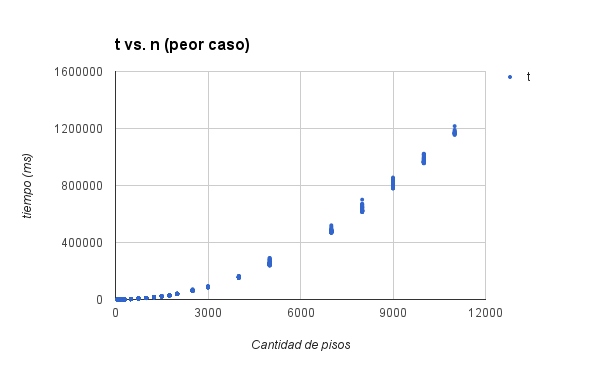
\includegraphics[width=11cm]{imagenes/ej1/tvsn-peorcaso.png}
	\caption{Relación entre tiempo de ejecución y cantidad de pisos (peor caso).}
	\label{tvsn-peorcasoB}
   \end{center}
 \end{figure}
\begin{figure}[h!]
   \begin{center}
 	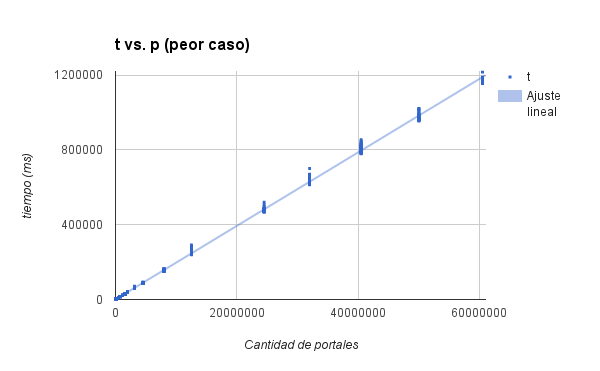
\includegraphics[width=11cm]{imagenes/ej1/tvsp-peorcaso.png}
	\caption{Relación entre tiempo de ejecución y cantidad de portales (peor caso).}
	\label{tvsp-peorcasoB}
   \end{center}
 \end{figure}

 
 Como se puede apreciar en los gráficos, el crecimiento de los tiempos de ejecución coincide con la complejidad calculada de forma analítica.